\documentclass[a3paper,12pt]{article}

\usepackage[left=2cm, right=2cm, top=2cm, bottom=2cm]{geometry} % Настройка отступов

\usepackage{graphicx} % Для работы с изображениями
\usepackage{caption} % Для настройки подписей к рисункам
\usepackage[russian]{babel} % Для русской локализации
\usepackage[utf8]{inputenc} % Для кодировки UTF-8
\usepackage[labelsep=period]{caption} % Устанавливает точку после номера рисунка



\begin{document}
\section*{Приложение}
\begin{figure}[htpb]
	\centering
	\setcounter{figure}{29}
	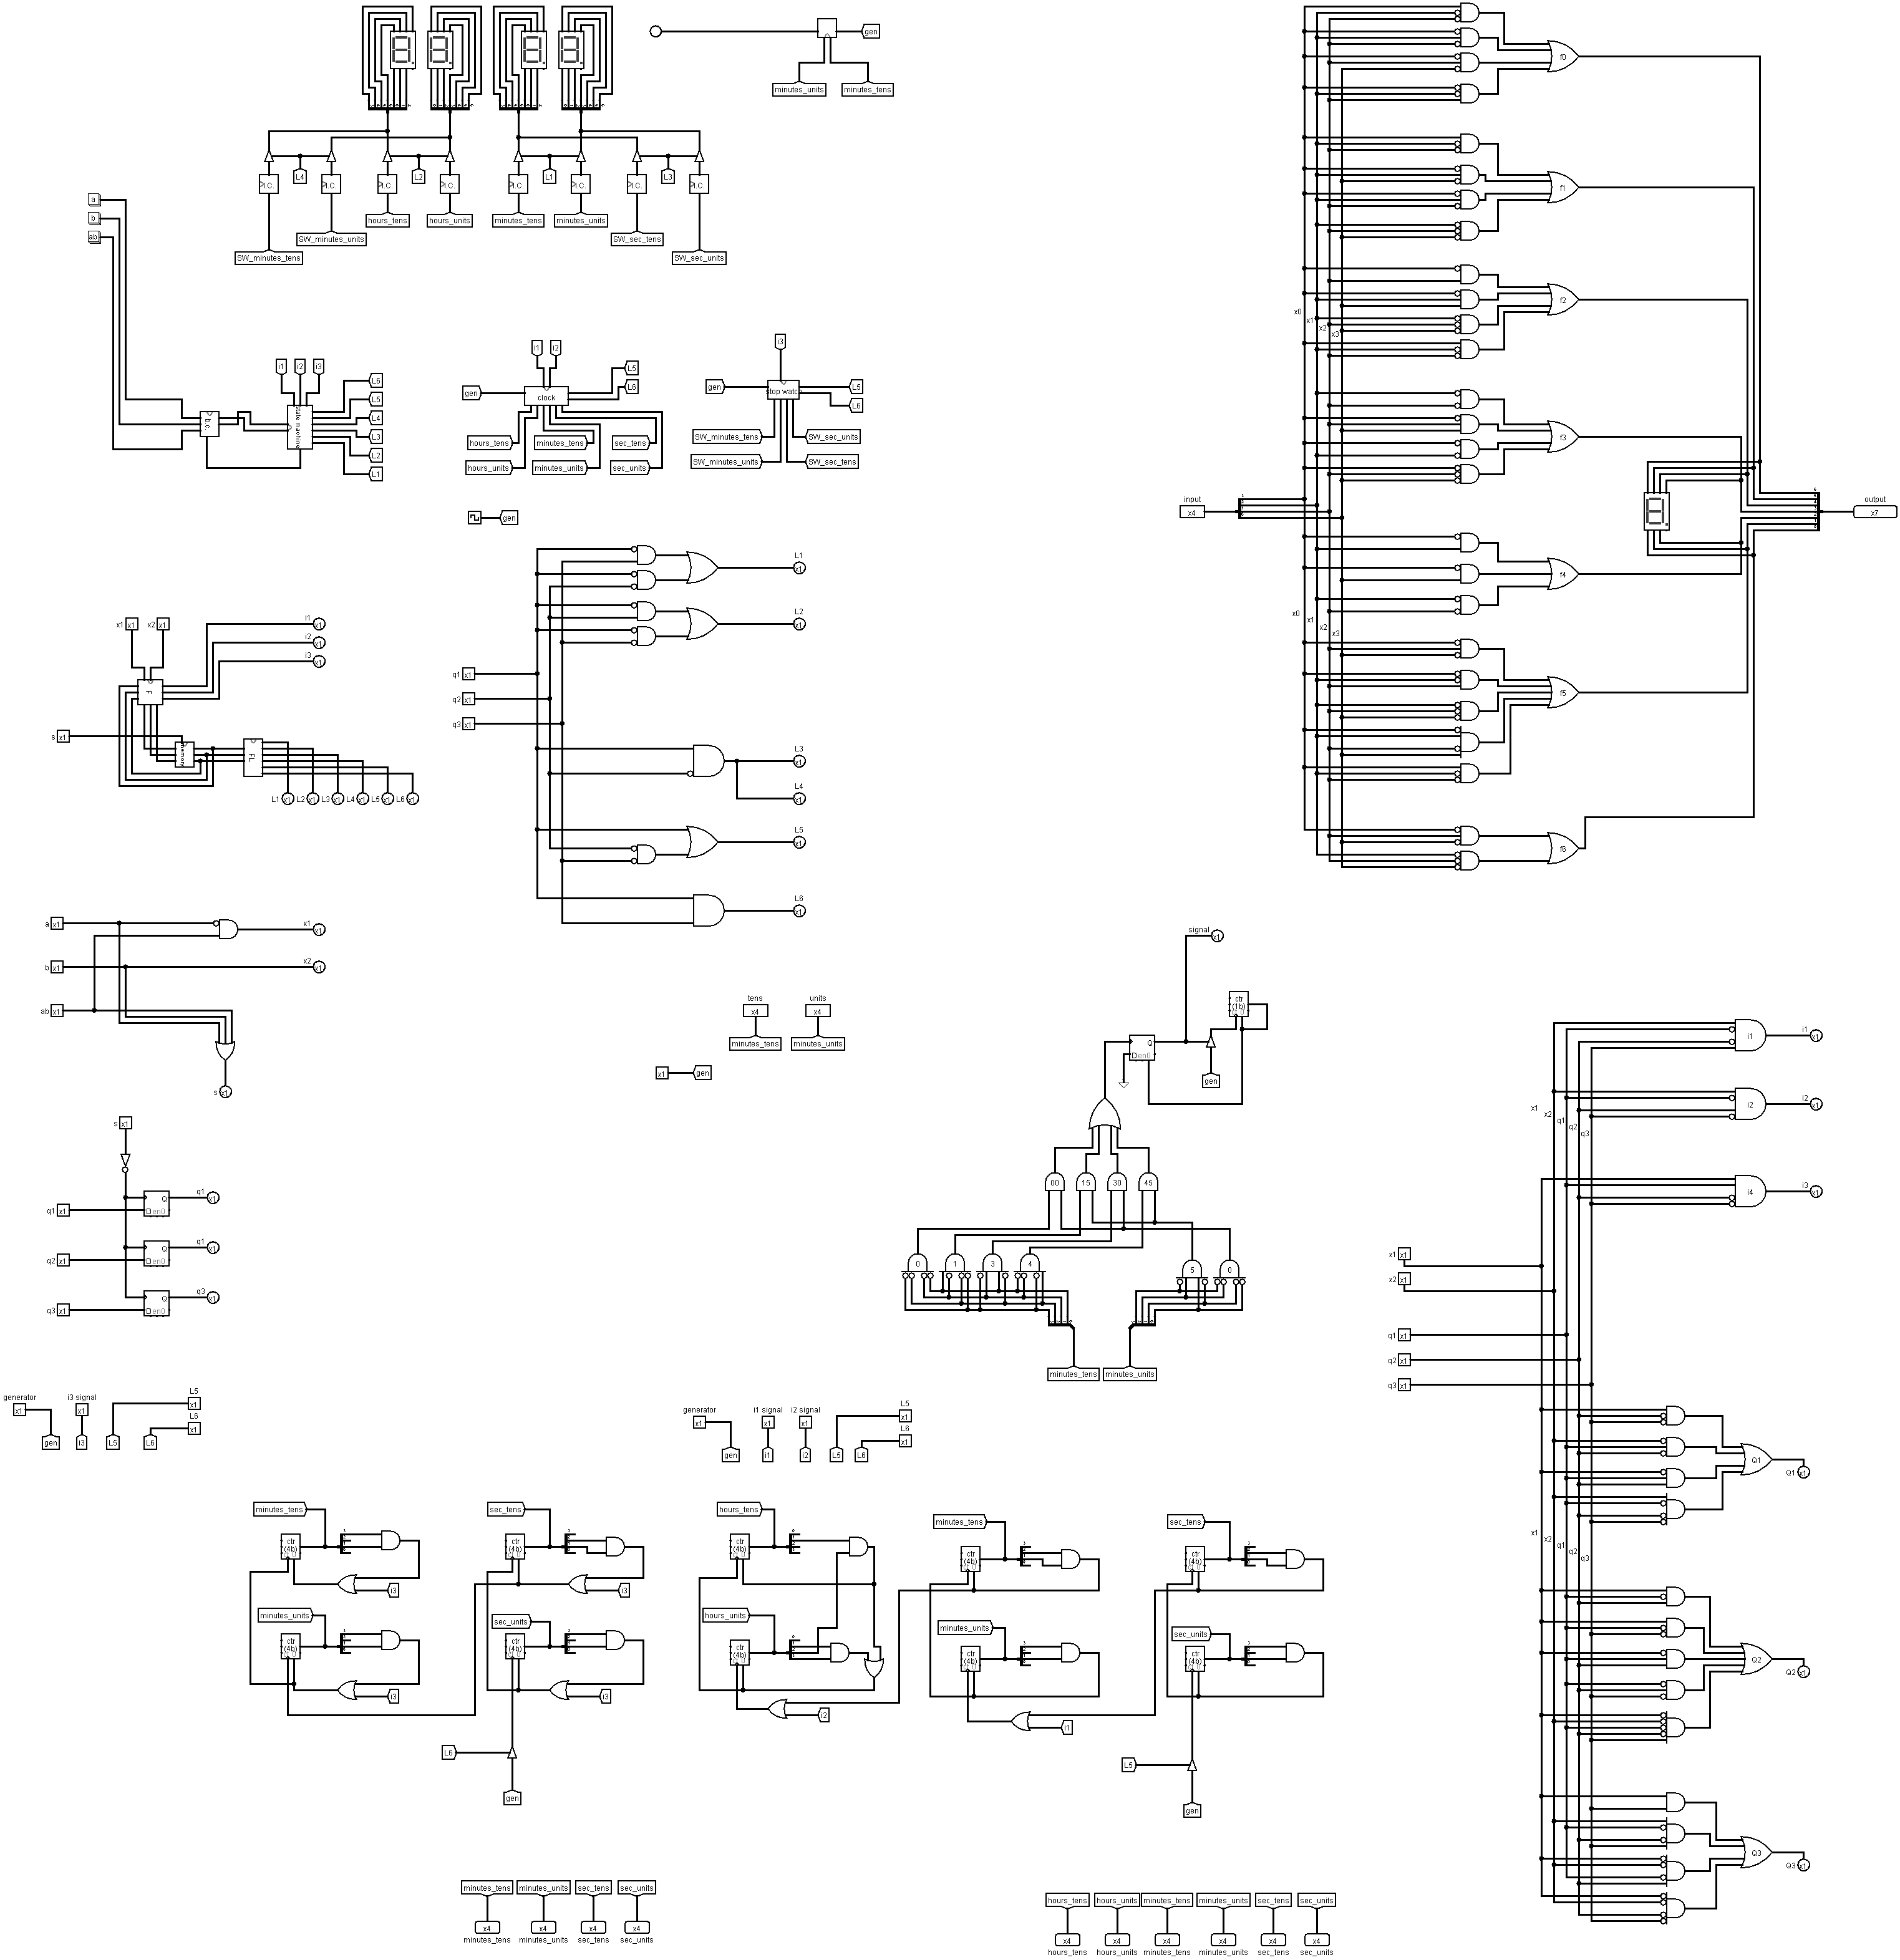
\includegraphics[scale=0.25]{logisim/img/functional scheme.png}
	\label{functional scheme} 
	\caption {Функциональная схема электронных часов }
\end{figure}
	
\end{document}